\documentclass[tikz,border=5pt]{standalone}
\usepackage[utf8]{inputenc}
\usepackage{tikz}
\usetikzlibrary{shapes.geometric, arrows.meta, positioning, shadows.blur, calc}

\definecolor{queryGold}{RGB}{243, 156, 18}
\definecolor{logicGray}{RGB}{127, 140, 141}
\definecolor{checkRed}{RGB}{192, 57, 43}
\definecolor{finalGreen}{RGB}{39, 174, 96}

\tikzset{
    base/.style={rectangle, rounded corners=2mm, text centered, font=\sffamily\small, draw=gray!40, thick, fill=white, blur shadow},
    proc/.style={base, minimum width=4cm, minimum height=1cm, text width=3.8cm},
    decision/.style={diamond, aspect=2, draw=checkRed!80!black, fill=checkRed!10, text width=2.5cm, font=\sffamily\tiny\bfseries, text centered},
    arrow/.style={-{Stealth}, thick, draw=gray!60}
}

\begin{document}
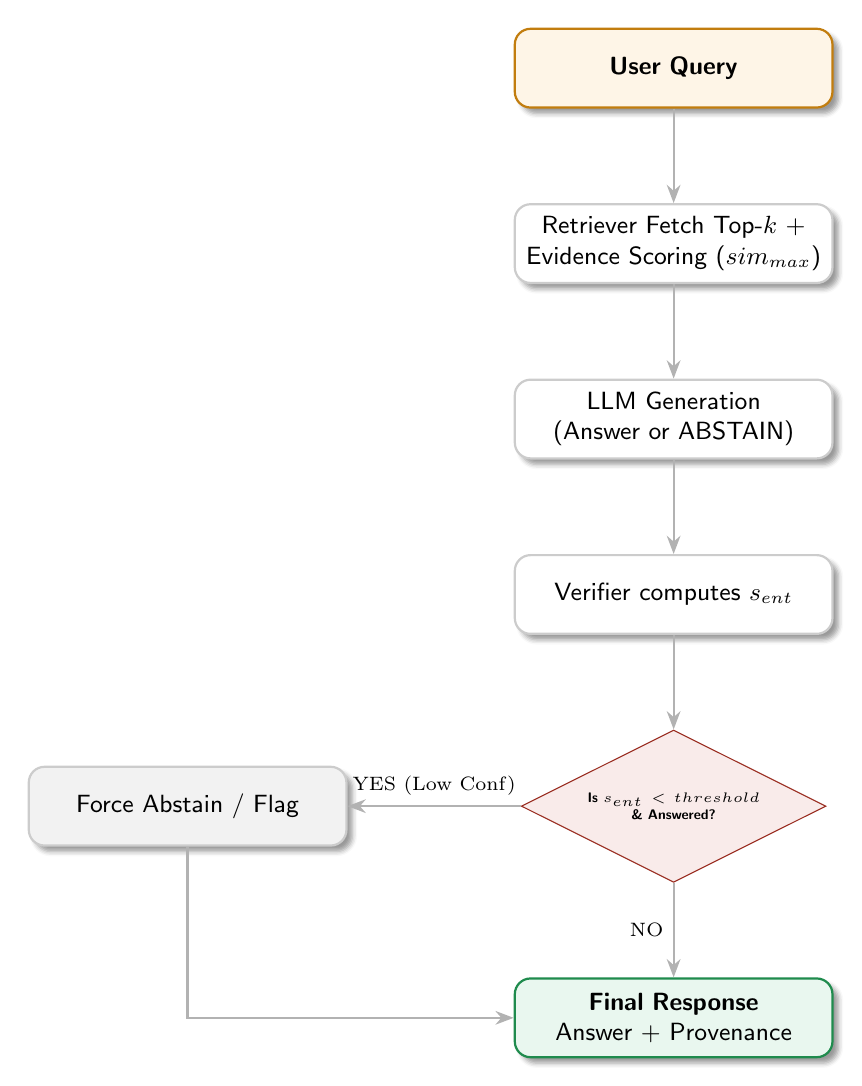
\begin{tikzpicture}[node distance=1.2cm]

    % Vertical Flow
    \node (start) [proc, fill=queryGold!10, draw=queryGold!80!black] {\textbf{User Query}};
    
    \node (fetch) [proc, below=of start] {Retriever Fetch Top-$k$ + Evidence Scoring ($sim_{max}$)};
    
    \node (llm) [proc, below=of fetch] {LLM Generation \\ (Answer or ABSTAIN)};

    \node (verify) [proc, below=of llm] {Verifier computes $s_{ent}$};

    % Decision Gate
    \node (gate) [decision, below=of verify] {Is $s_{ent} < threshold$ \& Answered?};

    % Outcomes
    \node (abstain) [proc, left=of gate, xshift=-1cm, fill=gray!10] {Force Abstain / Flag};
    
    \node (final) [proc, below=of gate, fill=finalGreen!10, draw=finalGreen!80!black] {
        \textbf{Final Response} \\ 
        Answer + Provenance
    };

    % Connecting
    \draw [arrow] (start) -- (fetch);
    \draw [arrow] (fetch) -- (llm);
    \draw [arrow] (llm) -- (verify);
    \draw [arrow] (verify) -- (gate);
    
    \draw [arrow] (gate) -- node[anchor=south, font=\scriptsize] {YES (Low Conf)} (abstain);
    \draw [arrow] (gate) -- node[anchor=east, font=\scriptsize] {NO} (final);
    
    \draw [arrow] (abstain) |- (final);

\end{tikzpicture}
\end{document}